\chapter{基于多传感器的无人机自主着舰系统实验验证}

\section{仿真实验环境构建}
\subsection{基于Matlab/Simulink的控制系统仿真环境实现}
Matlab软件于1980年由美国New Mexico大学的研究者Cleve Moler开发,其中Simulink是重要组件之一,该组件能够完成动态系统建模、仿真与综合分析等功能。为验证无人机底层控制和顶层控制算法,本文使用Simulink中的相关模块来完成仿真环境搭建。其中底层控制回路的仿真框图如图\ref{fig:chp08_07_matlab_control}所示,其中\texttt{Autopilot}模块主要完成底层控制,满足无人机的姿态控制需求。

\begin{figure}[!ht]
	\centering
	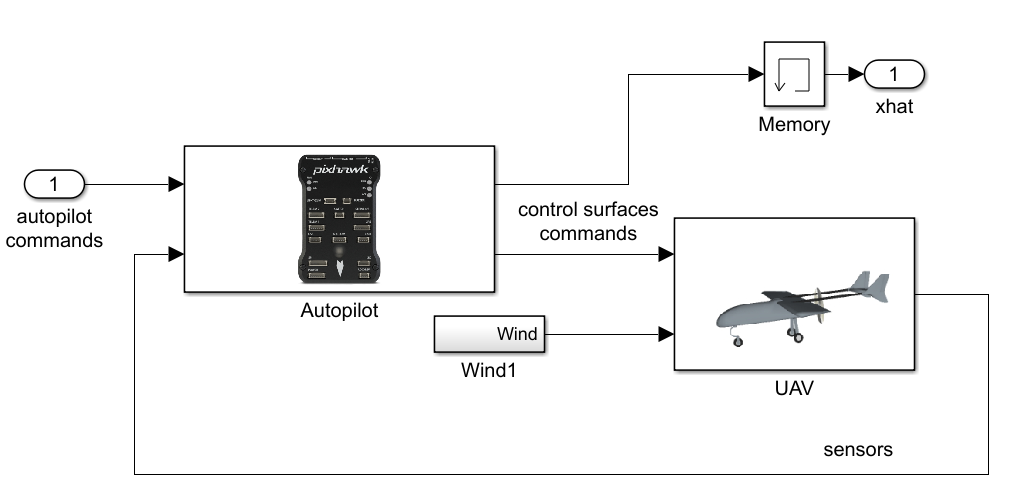
\includegraphics[width=0.8\textwidth]{figs/chp08/chp08_07_matlab_control.pdf}	
	\caption{Matlab/Simulink底层控制回路仿真}
	\label{fig:chp08_07_matlab_control}
\end{figure}

路径规划与顶层控制回路的仿真框图如图\ref{fig:chp08_06_matlab_sitl}所示,其中\texttt{Path Planner}模块主要产生基于Dubins Path的降落曲线,\texttt{Path Manager}模块主要判断降落曲线中的离散航点是否达到,\texttt{Path Follower}模块主要使用NMPC和TECS方法完成对降落曲线的跟踪,将底层控制指令传递给\texttt{Pixhawk}模块。

\begin{figure}[!ht]
	\centering
	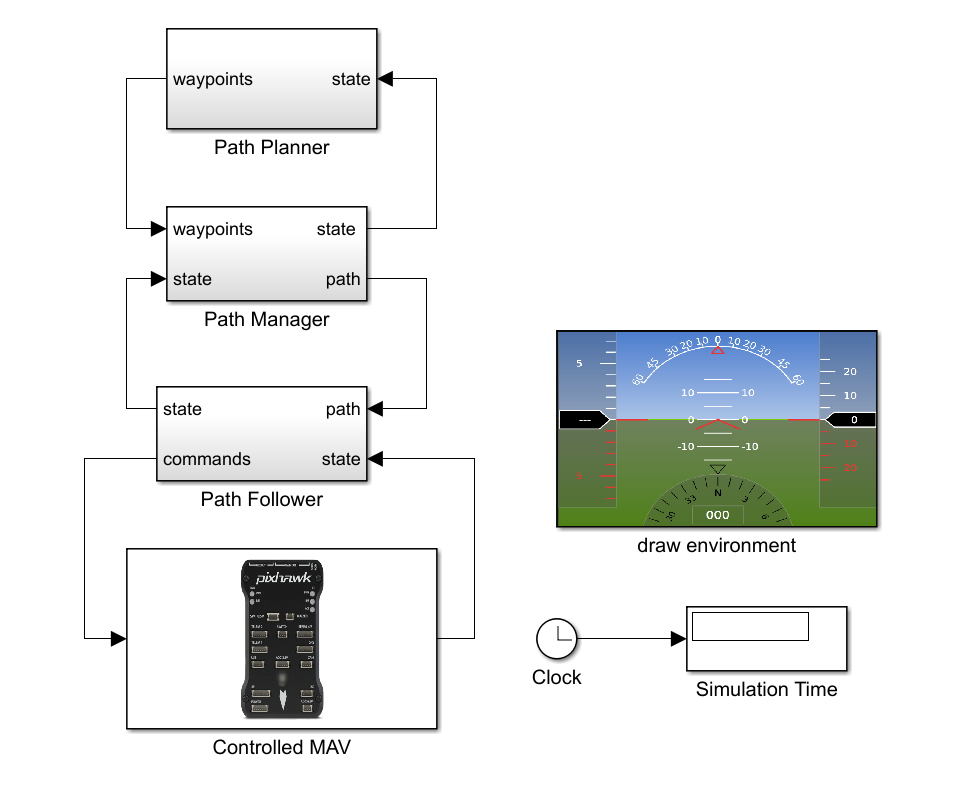
\includegraphics[width=0.7\textwidth]{figs/chp08/chp08_06_matlab_sitl.pdf}	
	\caption{Matlab/Simulink路径规划仿真}
	\label{fig:chp08_06_matlab_sitl}
\end{figure}

本文在是基于美国杨百翰大学(Brigham Young University,BYU)的研究者Randy Beard于2012年出版的《Small Unmanned Aircraft: Theory and Practice》一书\cite{beard2012small}中提供的Matlab/Simulink仿真环境基础之上修改完成。主要根据本文提出的降落曲线生成和控制算法对原有程序中的相应模块进行修改或重新设计。

\subsection{基于ROS和Gazebo的仿真环境实现}
ROS是Willow Garage公司在2010年发布的专门用于机器人研究和开发的操作系统。该操作系统最早起源于斯坦福大学,主要针对PR2机器人的需求进行设计。随着近年来机器人研究领域的持续升温,ROS系统越来越受到学术界和工业界的重视。ROS最重要的特点是解决了代码复用和模块化开发的需求。此外,ROS并不是传统意义上的操作系统,它的主体运行环境为Linxu系统,但其能够提供类似传统操作系统的诸多功能,例如硬件层的抽象描述、底层驱动程序的管理、驱动模块的共用、消息传递机制、程序的发行与管理和支持多种开发语言等。ROS中最重要的概念是节点(Nodes),这些节点通过消息的发布(Publish)和订阅(Subscribe)机制完成程序之间对数据的传递。

Gazebo仿真环境是独立于ROS系统的一套优秀的仿真软件。通过Gazebo仿真环境可以构建三维模型,能够定义物体的运动学和动力学参数,从而构建所需要的机器人单体、驱动模块、传感器模块和周边环境等。此外,Gazebo的插件(Plugin)开发完全开发,使用者可以根据自己的特殊需求修改和定制相应的仿真模块以满足实验要求。

由于ROS与Gazebo之间的数据交互工作可以通过编写特定的插件满足,因此越来越多的机器人研究者使用上述两个软件开展程序和算法初期开发和仿真测试。其中最为有名的两个应用场景是:(1)从2012年至2015年,由美国国防先进研究项目局设置的机器人挑战赛(DARPA Robotics Challenge,DRC)\cite{gazebo_darpa};(2)2016年度,由美国国家航空航天局设置的太空机器人挑战赛(NASA's Centennial Challenges: Space Robotics Challenge)\cite{gazebo_nasa}。由此,本文选择使用Gazebo与ROS的组合作为仿真环境的搭建。

考虑到Gazebo环境中对水面模拟需要耗费大量运算资源,因此设计使用地面移动平台来模拟舰船的运动。地面移动机器人上配置左右引导系统,该引导单元由两个矩形关节组合而成,具备二自由度独立运动能力并搭载不同型号的传感器,如图\ref{fig:chp08_02_ugv_gazebo}所示。图中左侧是地面移动平台和机基线距离为$5 \m$时的配置情况,右侧是地面移动平台的控制界面。通过该界面或者通过端口\texttt{/polaris/cmd\_vel}即可对地面移动平台进行手动控制或自主轨迹控制,由此实现模拟舰船在海面的平稳运动。此外,通过在引导系统的输出引入噪声,以此实现在不同海况扰动下的模拟。其中可见光传感器和红外传感器的参数可以在文件\texttt{gazebo\_camera\_plugin.cpp}和\texttt{polaris\_description/models/model-1\_4\_with\_ptu.sdf}中修改。

\begin{figure}[!t]
	\centering
	\includegraphics[width=\textwidth]{figs/chp08/chp08_02_ugv_gazebo.pdf}	
	\caption{Gazebo仿真环境下的地面移动机器人和引导系统与地面移动机器人操作界面}
	\label{fig:chp08_02_ugv_gazebo}
\end{figure}

对于无人机的模拟本文采用小型尺寸的无人机模型进行模拟,主要针对无人机的电机、副翼、襟翼、方向舵和升降舵进行设置。其中无人机机体模型和空气动力学参数根据第二章中的模型进行设计,具体参数详见文件\texttt{gazebo\_aerodynamics\_plugin.cpp}。在Gazebo环境中的无人机模型如图\ref{fig:chp08_04_gazebo_uav}所示,图中表示了无人机的基本控制机构,其中包含了副翼、襟翼、方向舵、升降舵和电机共五个控制量。

\begin{figure}[!ht]
	\centering
	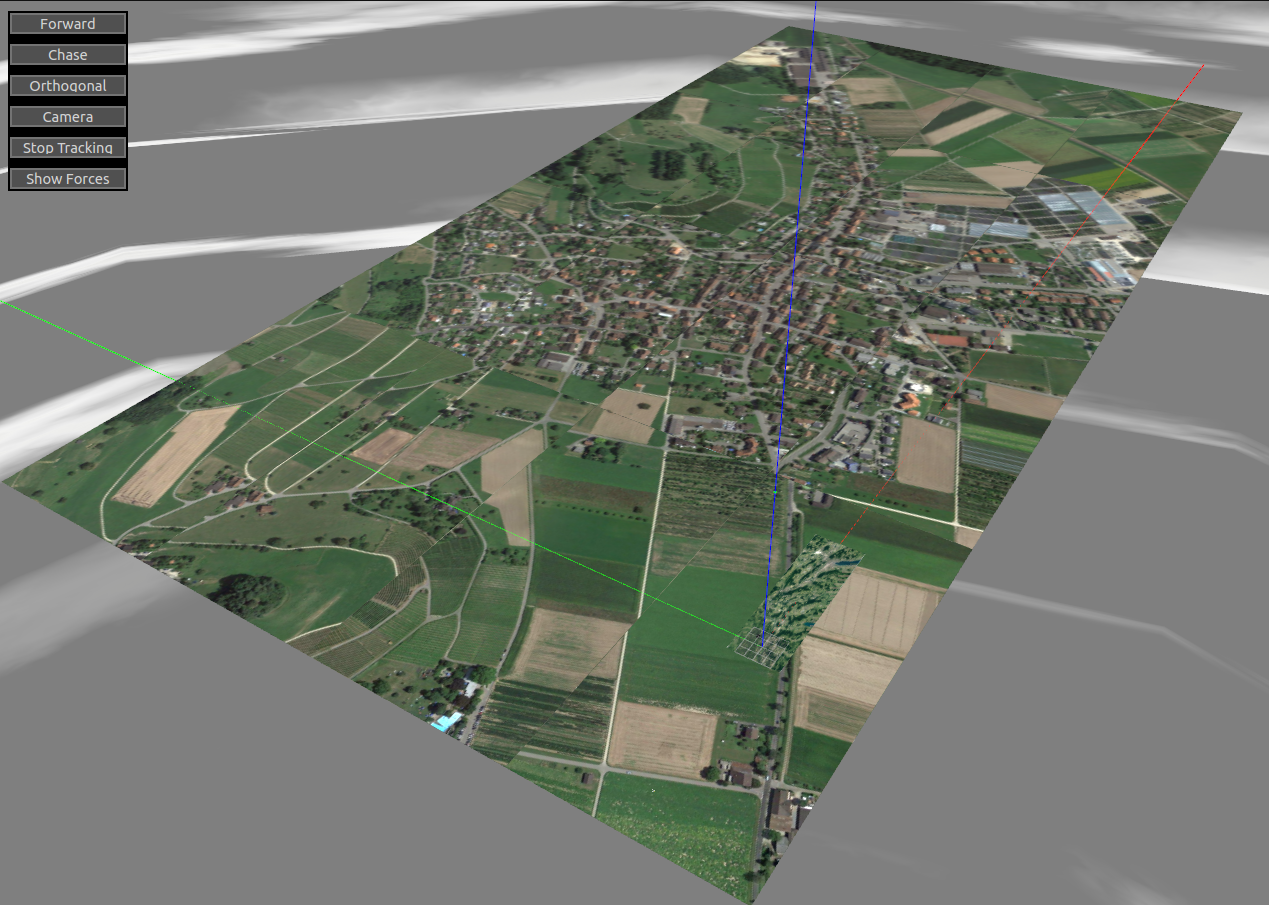
\includegraphics[width=0.7\textwidth]{figs/chp08/chp08_03_gazebo_landing_area.pdf}	
	\caption{Gazebo仿真环境下的无人机飞行区域}
	\label{fig:chp08_03_gazebo_landing_area}
\end{figure}

此外,为了更好的模拟飞行环境,本文替换了Gazebo原始环境中的地图,并引入风速扰动插件\texttt{gazebo\_wind\_plutin.cpp}来模拟飞行过程中的侧风扰动。图\ref{fig:chp08_04_gazebo_uav}所示为无人机在Gazebo中的仿真飞行场景。仿真环境中的主要节点名称和数据内容含义如图\ref{lab:ros_nodes_list}所示。

\begin{figure}[!ht]
	\centering
	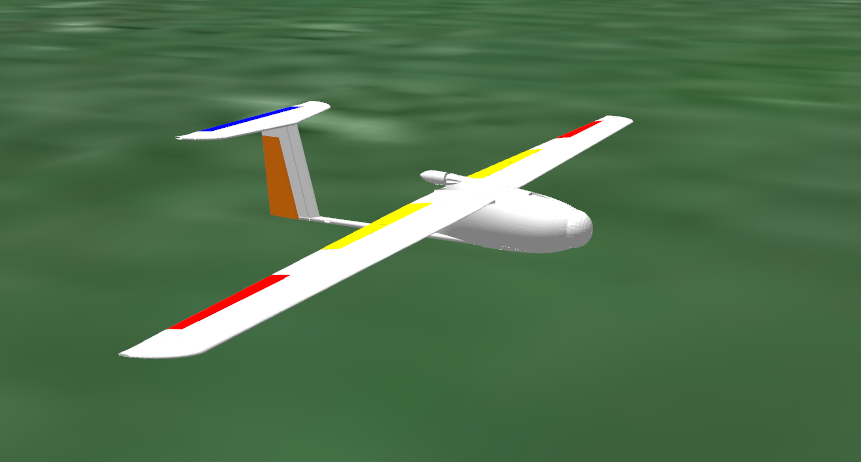
\includegraphics[width=0.7\textwidth]{figs/chp08/chp08_04_gazebo_uav.pdf}	
	\caption{Gazebo仿真环境下的小型固定翼无人机示意图}
	\label{fig:chp08_04_gazebo_uav}
\end{figure}

\begin{figure}[!ht]
	\centering
	\includegraphics[height=0.9\textheight]{figs/chp08/chp08_01_rosgraph.pdf}	
	\caption{ROS仿真环境中全部节点关系示意图}
	\label{fig:chp08_01_rosgraph}
\end{figure}

% Please add the following required packages to your document preamble:
% \usepackage{multirow}
% \usepackage{graphicx}
\begin{table}[!ht]
	\centering
	\caption{ROS与Gazebo仿真环境中核心节点的名称和数据内容定义}
	\label{lab:ros_nodes_list}
	\resizebox{\textwidth}{!}{%
		\begin{tabular}{clc}
			\hline
			& \multicolumn{1}{c}{\textbf{节点名称}} & \textbf{数据内容定义} \\ \hline
			\multirow{5}{*}{\begin{tabular}[c]{@{}c@{}}\textbf{左侧引导}\\ \textbf{单元节点}\end{tabular}} & /blackfly\_left/camera\_info & 相机标定参数 \\
			& /blackfly\_left/image\_raw & 相机原始图像 \\
			& /blackfly\_left/image\_raw/compressed & 相机压缩图像 \\
			& /left\_ptu/joint\_state & 转台当前姿态 \\
			& /left\_ptu/joint\_state\_cmd & 转台控制指令 \\ \hline
			\multirow{5}{*}{\begin{tabular}[c]{@{}c@{}}\textbf{右侧引导}\\ \textbf{单元节点}\end{tabular}} & /blackfly\_right/camera\_info & 相机标定参数 \\
			& /blackfly\_right/image\_raw & 相机原始图像 \\
			& /blackfly\_right/image\_raw/compressed & 相机压缩图像 \\
			& /right\_ptu/joint\_state & 转台当前姿态 \\
			& /right\_ptu/joint\_state\_cmd & 转台控制指令 \\ \hline
			\multirow{8}{*}{\begin{tabular}[c]{@{}c@{}}\textbf{无人机传感器}\\ \textbf{和控制量}\\ \textbf{节点}\end{tabular}} & /techpod/air\_pressure & 空气压力 \\
			& /techpod/air\_speed & 空速 \\
			& /techpod/camera & 机载相机图像 \\
			& /techpod/command/motor\_speed & 电机控制量 \\
			& /techpod/imu & 机载IMU数据 \\
			& /techpod/magnetic\_field & 机载磁罗盘数据 \\
			& /techpod/rotors\_key\_telop & 四个舵面和电机控制量 \\
			& /techpod/gps & 无人机GPS数据 \\ \hline
			\multirow{7}{*}{\begin{tabular}[c]{@{}c@{}}\textbf{无人机}\\ \textbf{真实值}\\ \textbf{节点}\end{tabular}} & /techpod/gazebo/wind\_speed & 环境风扰动 \\
			& /techpod/ground\_speed & 无人机地速 \\
			& /techpod/ground\_truth/imu & 无人机IMU数据 \\
			& /techpod/ground\_truth/odometry & 无人机里程计 \\
			& /techpod/ground\_truth/pose & 无人机姿态 \\
			& /techpod/ground\_truth/pose\_with\_covariance & 无人机姿态方差矩阵 \\
			& /techpod/ground\_truth/position & 无人机载惯性系的坐标 \\ \hline
			\multirow{3}{*}{\begin{tabular}[c]{@{}c@{}}\textbf{地面移动}\\ \textbf{平台节点}\end{tabular}} & /polaris/cmd\_vel & 地面移动平台控制量 \\
			& /polaris/odom & 地面移动平台里程计 \\
			& /polaris/ground\_truth/position & 地面移动平台在惯性系的位置 \\ \hline
		\end{tabular}%
	}
\end{table}

根据上述软件设计,即可完成无人机的软件在回路仿真。为了验证Pixhawk和Odroid XU4的工作性能,可以进一步将ROS和Gazebo的数据通过串口传递给Pixhawk和Odroid XU4,以此达到硬件在回路仿真测试的结果。两种仿真环境的构建框图如图\ref{fig:chp08_05_SITL_HITL}所示。其中软件在回路仿真的蓝色模块可以与硬件在回路仿真的蓝色模块相互替换,以此满足相应的仿真需求。

\begin{figure}[!ht]
	\centering
	\includegraphics[width=\textwidth]{figs/chp08/chp08_05_SITL_HITL.pdf}	
	\caption{硬件在回路仿真和软件在回路仿真示意图}
	\label{fig:chp08_05_SITL_HITL}
\end{figure}

上述综合系统是基于瑞士苏黎世联邦理工学院(Eidgenössische Technische Hochschule Zürich,ETH)自主控制研究实验室(Autonomous System Lab,ASL)开发的RotorS\cite{Furrer2016}仿真环境中进一步开发过程中得到,其中主要添加了地面移动平台和控制系统、车载多传感器引导系统和无人机控制模块等。改造后的程序发布在\texttt{https://github.com/weiweikong/rotors\_simulator}。



\section{外场实验环境构建}
为实现全天候,高精度,复杂应用情况下的通用无人机自主起降引导系统。具有快速展开、模块化、方便集成以及高效的多传感器融合的特点,具体需要实现以下功能指标:
(1)能够对云台进行手动和自动控制的切换,以满足对系统标定、算法测试、快速对准等方面的需求。
(2)能够适应能见度较差的天气情况,具备在可见光和近红外相机之间进行快速切换功能。
(3)在无人机距离期望引导位置大于一公里时,能够通过红外相机和UWB能够使得转台准确跟踪目标。
(4)引导系统的相对定位精度为:水平方向≤0.5m,高度方向≤0.2m。
(5)最大探测距离不低于2km(翼展5米无人机),最大探测距离不低于1km(翼展3米无人机)。

\subsection{转台选型}
引导系统使用的二自由度转台选用美国FLIR公司的双轴陀螺稳定转台,型号为PTU-D300。该转台支持通过RS232串口发送指令,并能实时反馈转台状态,包括转台的方位角(Pan)和俯仰角(Tilt)。转台的分辨率为$0.006\degree$ 。该转台外形如图\ref{fig:chp08_08_PTU-D300E_large}所示。PTU-D300为步进电机驱动,能够满足闭环跟踪目标的需求。转台抗振动冲击较好,防护等级IP67,支持野外、舰船、车载等恶劣工作环境。具体参数可参考表\ref{lab:FLIR_D300}。该转台的两侧可以安装负载支架,支持多种安装模式,为多种传感器的安装提供搭载平台。
\begin{figure}[!ht]
	\centering
	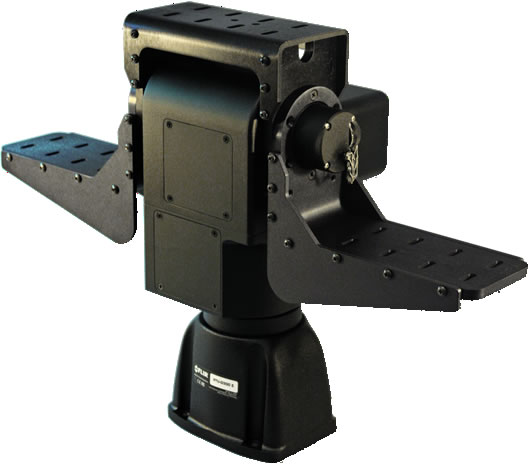
\includegraphics[width=0.4\textwidth]{figs/chp08/chp08_08_PTU-D300E_large.pdf}	
	\caption{FLIR D300转台}
	\label{fig:chp08_08_PTU-D300E_large}
\end{figure}
% Please add the following required packages to your document preamble:
% \usepackage{graphicx}
\begin{table}[!ht]
	\centering
	\caption{FLIR D300转台性能指标}
	\label{lab:FLIR_D300}
	\begin{tabular}{cc}
		\hline
		& \textbf{性能指标}                                                                                                          \\ \hline
		\textbf{运动性能} & \begin{tabular}[c]{@{}c@{}}航向角:$360\degree$连续旋转\\ 俯仰角:$-90\degree-30\degree$\end{tabular}                              \\
		\textbf{转动速度} & $0.064\degree/s-50\degree/s$                                                                                           \\
		\textbf{负载能力} & $18.1\ kg$                                                                                                             \\
		\textbf{电源输入} & DC$12-30$ V                                                                                                            \\
		\textbf{工作温度} & $-30\degree C-70\degree C$                                                                                             \\
		\textbf{步进模式} & \begin{tabular}[c]{@{}c@{}}1/2 STEP: $0.020\degree$\\ 1/4 STEP: $0.012\degree$\\ 1/8 STEP: $0.006\degree$\end{tabular} \\ \hline
	\end{tabular}
\end{table}

当无人机的飞行速度为$30\ m/s$,距离引导系统为$200\ m$时,转台所需要的转动速度为$4.3\ \degree/s$,该数值属于转台的正常工作范围。此外,无人机降落过程中,在不确定进场方向的情况下,转台方位角的工作范围能做使得引导系统具备全空域搜索能力。此外,为防止在转台转动过程中底座发生移动,为此在转台底部设计了可调式三角稳定底座,机械结构如图\ref{fig:chp08_10_ptu_with_sensor}所示。因此,该转台系统具有较强的负载能力和较好的调节精度,可以满足引导系统的工作要求。如图所示,可以根据需要对传感器进行配置。图中左侧的是可见光和红外光相机的组合,右侧为红外光相机、激光照射器和UWB雷达的组合方式。

\begin{figure}[!t]
	\centering
	\includegraphics[width=0.8\textwidth]{figs/chp08/chp08_10_ptu_with_sensor.pdf}	
	\caption{FLIR D300搭载不同传感器的配置方式和支撑系统}
	\label{fig:chp08_10_ptu_with_sensor}
\end{figure}


\subsection{可见光相机}
可见光相机的选型为Imaging Source公司的彩色CCD高速工业像机,型号为DFK 23G445,接口为GigE。该相机使用的CCD芯片为Sony ICX445AQA,其像素分辨率为$640\times480$,像元尺寸为$5.6\  \mu m$,最大帧频为$30\ fps$。该相机使用GigE接口,使得仅适用一根网线即可承担供电和数据传送的双重功能,能够满足远距离配置系统和图像信息高速传递的需求。

\begin{figure}[!ht]
	\centering
	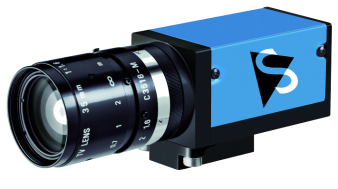
\includegraphics[width=0.4\textwidth]{figs/chp08/chp08_11_imagingsource_camera.pdf}	
	\caption{The Imaging Source 彩色相机}
	\label{fig:chp08_11_imagingsource_camera}
\end{figure}

对于镜头的选择,本文选用$100\ mm$焦距镜头,该镜头后的视场角为$1.936\degree \times 1.452 \degree$。深度方向距离为$400\ m$时,探测窗口大小约为$13.5\times10.1\ m$;深度方向距离为$800\ m$时,探测窗口大小约为$27.0\times20.2\ m$。对于实验中使用的中型无人机而言,该无人机的翼展为$3\ m$,其在$800\ m$处的理论成像像素为$71\ pixel$。本文使用的目标识别算法能够对该距离的目标进行有效识别。

\subsection{电台设备}	
由于需要将舰载引导系统的信息回传给无人机导航系统,因此需要选择合适的电台。本文选用的是加拿大Microhard公司的Nano IP系列的IPn 920,如图所示。该电台具有尺寸小、低功耗、传输可靠、能远距离快速通信等优势。其工作频率为$902-928\ MHz$,具有$1.2\ Mbps$的传输速率。此外该电台还具备自动组网,点对点(P2P)、点对多点(P2E)、任意点对任意点(E2E)等多种组网模式,同时支持网络、两路串口通信,上述指标能够满足无人机降落过程中的引导信息上传和无人机信息下传的需求。

\begin{figure}[!ht]
	\centering
	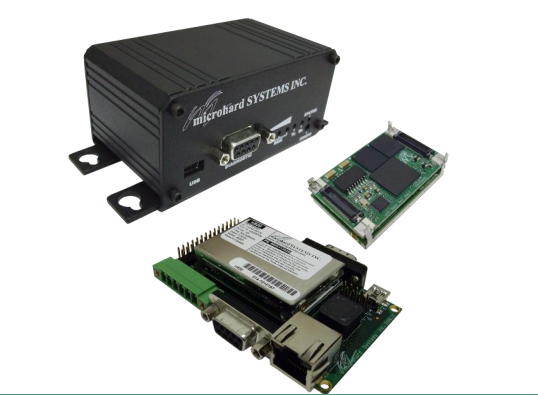
\includegraphics[width=0.5\textwidth]{figs/chp08/chp08_12_micohard_radio.pdf}	
	\caption{Microhard公司的IPn 920电台}
	\label{fig:chp08_12_micohard_radio}
\end{figure}

\subsection{无人机平台}

对于小型固定翼无人机平台而言,本文选用经典的“天行者“平台,如图\ref{fig:chp08_13_small_sized_uav}所示。该平台的翼展为$1880\ mm$,有效载荷为$2\ kg$,平均飞行时间为$40 \min$,最大飞行速度为$90\ km/h$,最小飞行速度为$35\ km/h$。该飞机的机舱相对较小,但能够满足加装Pixhawk自驾仪和Odroid XU4开发版的需求。仿真环境中所模拟的无人机尺寸与该小型固定翼无人机平台参数基本相同,本文使用的小型固定翼无人机降落数据集由该平台产生。

\begin{figure}[!ht]
	\centering
	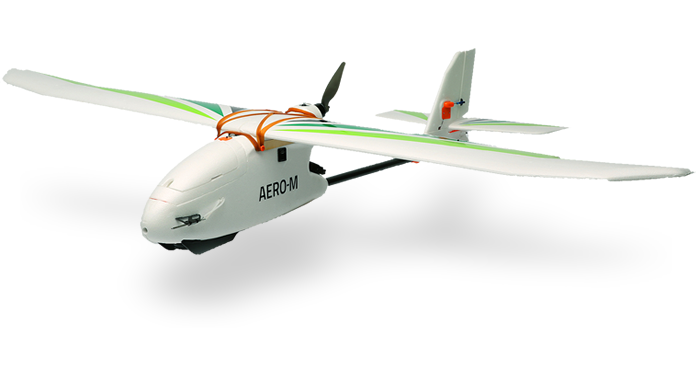
\includegraphics[width=0.6\textwidth]{figs/chp08/chp08_13_small_sized_uav.pdf}	
	\caption{“天行者”小型固定翼无人机}
	\label{fig:chp08_13_small_sized_uav}
\end{figure}

对于中型固定翼无人机平台,本文选用后置发动机的“开拓者”无人机平台。该平台选用前三点式双尾撑布局如图\ref{fig:chp08_14_middle_sized_uav}所示。“开拓者”无人机长$2200\ mm$,翼展$3000\ mm$,重量为$20\ kg$,巡航速度$120\ km/h$。最初,为提升视觉检测的可靠性,选用涂装为橙色的“开拓者”无人机,便于在复杂背景下检测跟踪目标。由于本文最终所采用的图像跟踪算法使用的是灰度图像,因此跟踪算法识别精度和跟踪速度对涂装颜色不敏感,同时,为了配合激光照射模块,在其机头处安装了反射棱镜作为合作目标。本文使用的中型固定翼无人机降落数据集由该平台产生。

\begin{figure}[!ht]
	\centering
	\includegraphics[width=0.8\textwidth]{figs/chp08/chp08_14_middle_sized_uav.pdf}	
	\caption{“开拓者”中型固定翼无人机}
	\label{fig:chp08_14_middle_sized_uav}
\end{figure}





\section{综合实验结果}
\subsection{地面环境引导系统测试实验设计}
根据上述设备选型,可以根据不同需求构建不同配置的引导系统。在2012年,首先通过普通安防转台和红外相机构建了第一版地基引导系统,如图\ref{fig:first_version_ptu}所示,该系统的基线长度为$0.25\ m$。由于转台的性能约束,该系统只能通过串口方式对俯仰角和横滚角进行控制,其两个方向的转动角度只能通过计算串口输出的控制指令得到,即通过开环的方式获得。该系统通过四旋翼无人机的飞行试验,初步验证了立体视觉系统与转台结合这一设计模式的可行性。该系统在户外对四旋翼目标进行引导降落的工作图如图\ref{fig:first_version_ptu_2}所示。

\begin{figure}[!t]
	\begin{minipage}{0.5\textwidth}
		\centering
		\includegraphics[width=0.98\textwidth]{figs/chp08/chp08_09_original_ptu.pdf}	
		\caption{第一版红外引导单元}
		\label{fig:first_version_ptu}
	\end{minipage}\hfill
	\begin{minipage}{0.5\textwidth}
		\centering
		\includegraphics[width=0.98\textwidth]{figs/chp08/chp08_15_OldSystem.pdf}	
		\caption{第一版引导系统工作图}
		\label{fig:first_version_ptu_2}
	\end{minipage}
\end{figure}

为提升转台性能,增强对无人机目标的检测能力和检测距离,2013年起引导系统开始采用FLIR D300型号转台,立体视觉的基线长度也增加为$0.45\ m$,该系统的引导单元构成如图\ref{fig:chp08_18_ground_short_ptus}左侧图像所示。得益于基线长度的增加,与第一版系统相比,该系统的检测距离可以得到$400\ m$,通过红外相机图像和可见光相机图像的融合使用,能够对没有合作标识的无人机有较好的跟踪和识别效果。该系统一般放置于跑道中心线位置,其工作场景如图\ref{fig:chp08_18_ground_short_ptus}所示。

\begin{figure}[!ht]
	\centering
	\includegraphics[width=\textwidth]{figs/chp08/chp08_18_ground_short_ptus.pdf}	
	\caption{第二版引导系统工作图}
	\label{fig:chp08_18_ground_short_ptus}
\end{figure}

第二版系统的检测能力和距离虽然有所提升,但由于其放置位置不适用于实际需求场景,同时,基线长度仍然无法满足对中型无人机的远距离降落的引导需求指标。因此,本文考虑突破原因固定基线物理机构的约束,通过将两个独立的引导单元进行独立配置,使得引导的基线距离能够根据物理场地约束和无人机尺寸大小进行最优配置。在基线长度为$10\  m$时,地面引导系统的配置情况如图\ref{fig:chp08_17_ground_ptus}所示。上述三个版本引导系统的具体参数和配置情况如表\ref{lab:three_ground_ptu}所示。

\begin{figure}[!t]
	\centering
	\includegraphics[width=\textwidth]{figs/chp08/chp08_17_ground_ptus.pdf}	
	\caption{第三版引导系统工作图}
	\label{fig:chp08_17_ground_ptus}
\end{figure}

\begin{table}[!t]
	\centering
	\caption{三版不同配置的地面引导系统}
	\label{lab:three_ground_ptu}
	\begin{tabular}{clll}
		\hline
		& \multicolumn{1}{c}{\textbf{布局模式}} & \multicolumn{1}{c}{\textbf{传感器系统}} & \multicolumn{1}{c}{\textbf{目标检测距离}} \\ \hline
		\textbf{\begin{tabular}[c]{@{}c@{}}第一版\\ 引导系统\end{tabular}} & \begin{tabular}[c]{@{}l@{}}普通安防转台 $\times$ 1\\ 基线长度 $0.25\ m$\end{tabular} & 远红外相机 $\times$ 2 & \begin{tabular}[c]{@{}l@{}}对MD4-200四旋翼无人机\\ 的检测距离为$90\ m$\end{tabular} \\ \hline
		\textbf{\begin{tabular}[c]{@{}c@{}}第二版\\ 引导系统\end{tabular}} & \begin{tabular}[c]{@{}l@{}}FLIR转台 $\times$ 1\\ 基线长度 $0.45\ m$\end{tabular} & \begin{tabular}[c]{@{}l@{}}远红外相机 $\times$ 2\\ 可见光相机 $\times$ 2\end{tabular} & \begin{tabular}[c]{@{}l@{}}对中型无人机的\\ 检测距离为$400\ m$\end{tabular} \\ \hline
		\textbf{\begin{tabular}[c]{@{}c@{}}第三版\\ 引导系统\end{tabular}} & \begin{tabular}[c]{@{}l@{}}FLIR转台 $\times$ 2\\ 基线长度可自由配置,\\ 一般为$10\ m$\end{tabular} & \begin{tabular}[c]{@{}l@{}}远红外相机 $\times$ 2\\ 可见光相机 $\times$ 2\\ 激光照射器 $\times$ 1\\ UWB雷达 $\times$ 1\end{tabular} & \begin{tabular}[c]{@{}l@{}}对中型无人机的\\ 检测距离为$1000\ m$\end{tabular} \\ \hline
	\end{tabular}
\end{table}


\subsection{地面引导降落实验结果}
地基无人机降落实验主要通过在地面配置基线为$10\ m$的引导系统完成。其基本就工作顺序如下:(1)飞机首先由飞行操作手起飞或自主起飞,在进入指定空域后,切换至依赖DGPS的航线飞行模式。一般为在跑道上空飞行训练航线,即四边航线。(2)在地面引导设备和飞行器工作状态正常的情况下,在飞机完成一次低空通场飞行后,启动引导系统的跟踪模式和飞机的降落模式。(3)无人机根据当前位置和期望降落位置对降落轨迹进行实施规划,一般在最后一个转弯时,能够被地面引导系统的视觉传感器捕获。(4)在引导数据的精读和更新速率满足条件后,在飞控端停止DGPS数据对位置信息的修正,只记录位置用于后续数据分析。无人机在该阶段的相对位置信息由地面引导系统提供,并完成最后降落。图\ref{fig:chp08_23_ground_landing}所示为其中一组在湖南长沙进行的地面引导无人机降落实验全过程示意图。
\begin{figure}[!th]
	\centering
	\includegraphics[width=\textwidth]{figs/chp08/chp08_23_ground_landing.pdf}	
	\caption{地面引导系统引导降落无人机回收过程图}
	\label{fig:chp08_23_ground_landing}
\end{figure}

图\ref{fig:chp08_23_ground_landing}的上半部分为降落过程中的四个重要时间节点,下半部分为实际飞行数据的轨迹和误差比较。其中紫色部分为地面引导系统提供有效引导信息的工作范围,该部分的三个坐标轴方向的误差在下半部分的右侧第一列所示,经过EKF方法之后的数据与DGPS数据的比较结果为右侧第二列所示。通过三维图示中的紫色视觉解算结果可以发现,尽管视觉系统可以有效跟踪无人机目标,且通过对转台信息进行了补偿,但其解算结果的波动依然较大。在使用EKF之后,数据的波动得到有效缓解,能够完成引导降落任务。

地面引导实验分别于2014年和2015年在湖南长沙和江西吉安共进行全系统测试,共完成八组测试,具体实验数据如表\ref{lab:eight_ground_landing}所示。 其中根据测试时的气象条件不同对实验数据进行分类统计,每一类别的最远检测距离和误差最小数值用粗体表示,最近检测距离和误差最大数值用下划线标注。通过图表可以发现气象条件对光学系统的检测距离影响依然较大,同时对三个方向的引导精度也产生了较大影响。通过第三章的分析可知,在远端的系统理论误差较大,随着目标进一步靠近引导系统,理论误差迅速变小,因此单纯比较一组实验的三个方向的平均引导精读说服力有限。

\begin{table}[]
	\centering
	\caption{八组不同气象条件下的实验结果}
	\label{lab:eight_ground_landing}
	\begin{tabular}{cccccc}
		\hline
		\multicolumn{1}{l}{\textbf{实验序号}} & \multicolumn{1}{l}{\textbf{光照条件}} & \multicolumn{1}{l}{\textbf{最远检测距离}} & \multicolumn{1}{l}{\textbf{RMSE $\mathbf{i}^{O,c}$(m)}} & \multicolumn{1}{l}{\textbf{RMSE $\mathbf{j}^{O,c}$(m)}} & \multicolumn{1}{l}{\textbf{RMSE $\mathbf{k}^{O,c}$(m)}} \\ \hline
		\textbf{1} & 晴天 & 848.735 & \underline{0.325} & \underline{1.451} & 0.280 \\
		\textbf{2} & 晴天 & \textbf{892.134} & 0.239 & 1.281 & \textbf{0.212} \\
		\textbf{3} & 晴天 & 872.311 & 0.373 & 1.319 & 0.282 \\
		\textbf{4} & 晴天 & \underline{847.373} & 0.259 & 1.401 & 0.233 \\
		\textbf{5} & 晴天 & 857.117 & \textbf{0.242} & \textbf{1.241} & \underline{0.301} \\ \hline
		\textbf{6} & 阴天 & \underline{491.193} & \underline{0.491} & 1.676 & \underline{0.599} \\
		\textbf{7} & 阴天 & 503.175 & 0.483 & \textbf{1.345} & \textbf{0.576} \\
		\textbf{8} & 阴天 & \textbf{534.238} & \textbf{0.470} & \underline{1.772} & 0.581 \\ \hline
	\end{tabular}
\end{table}

因此,本文统计了将引导距离以$20\ m$为单位进行切分,分段评估引导的效果,表\ref{lab:ground_landing}所示为不同阶段的引导系统在引导坐标系$\mathcal{O}_c$中三个坐标轴方向的平均误差。通过表中数据可以发现,深度方向$\mathbf{j}^{O,c}$方向的误差受视觉解算的引导误差相对较大,其他两个轴的误差相对较小。

\begin{table}[!th]
	\centering
	\caption{在距离降落点不同位置时,引导系统三个方向的平均误差}
	\label{lab:ground_landing}
	\begin{tabular}{cccc|cccc}
		\hline
		\textbf{Interval(m)} & \textbf{$\mathbf{i}^{O,c}$(m)} & \textbf{$\mathbf{j}^{O,c}$(m)} & \textbf{$\mathbf{k}^{O,c}$(m)} & \textbf{Interval(m)} & \textbf{$\mathbf{i}^{O,c}$(m)} & \textbf{$\mathbf{j}^{O,c}$(m)} & \textbf{$\mathbf{k}^{O,c}$(m)} \\ \hline
		\textbf{600$\sim$580} & 0.332 & 1.856 & 0.431 & \textbf{300$\sim$280} & 0.128 & 1.426 & 0.171 \\
		\textbf{580$\sim$560} & 0.311 & 1.434 & 0.371 & \textbf{280$\sim$260} & 0.123 & 1.313 & 0.159 \\
		\textbf{560$\sim$540} & 0.208 & 1.542 & 0.300 & \textbf{260$\sim$240} & 0.104 & 1.104 & 0.114 \\
		\textbf{540$\sim$520} & 0.182 & 1.569 & 0.276 & \textbf{240$\sim$220} & 0.086 & 0.612 & 0.129 \\
		\textbf{520$\sim$500} & 0.217 & 1.863 & 0.180 & \textbf{220$\sim$200} & 0.099 & 0.882 & 0.131 \\
		\textbf{500$\sim$480} & 0.209 & 1.049 & 0.216 & \textbf{200$\sim$180} & 0.162 & 0.933 & 0.157 \\
		\textbf{480$\sim$460} & 0.185 & 1.478 & 0.253 & \textbf{180$\sim$160} & 0.154 & 0.730 & 0.136 \\
		\textbf{460$\sim$440} & 0.198 & 1.245 & 0.243 & \textbf{160$\sim$140} & 0.134 & 0.922 & 0.201 \\
		\textbf{440$\sim$420} & 0.171 & 1.412 & 0.151 & \textbf{140$\sim$120} & 0.143 & 0.696 & 0.125 \\
		\textbf{420$\sim$400} & 0.186 & 1.674 & 0.119 & \textbf{120$\sim$100} & 0.172 & 0.900 & 0.118 \\
		\textbf{400$\sim$380} & 0.159 & 1.679 & 0.145 & \textbf{100$\sim$80} & 0.139 & 0.668 & 0.079 \\
		\textbf{380$\sim$360} & 0.153 & 1.527 & 0.197 & \textbf{80$\sim$60} & 0.170 & 0.696 & 0.067 \\
		\textbf{360$\sim$340} & 0.171 & 1.292 & 0.138 & \textbf{60$\sim$40} & 0.105 & 0.460 & 0.055 \\
		\textbf{340$\sim$320} & 0.164 & 1.360 & 0.217 & \textbf{40$\sim$20} & 0.126 & 0.276 & 0.082 \\
		\textbf{320$\sim$300} & 0.156 & 1.420 & 0.204 & \textbf{20$\sim$00} & 0.070 & 0.261 & 0.095 \\ \hline
	\end{tabular}
\end{table}


\subsection{水面环境引导系统测试实验设计}
根据上一小节的介绍,引导系统在水面上的设计方案是基于第三版进一步改进和完善。由于缺少舰船作为载体,本文通过使用油桶和脚手架搭建简易浮体来模拟在水面的浮体运动。该系统的设计图如图\ref{fig:chp08_22_landing_diagram}所示。图中中部的为浮体上的木板,平台大小约为$12\ m\times 12\ m$,中间位置安装高度为$8\ m$,宽度为$10\ m$的无人机回收网,为了避免回收网对视觉系统的干扰,在回收网前端设置两个引导单元。该浮体自身并无动力,在水面实验时,需要通过右侧的牵引船只通过缆绳对浮体进行拖动。浮体和设备整体重量相对较重,在江面实验时,只对牵引船只的运动方向进行设定,对运动速度不做要求。

\begin{figure}[!th]
	\centering
	\includegraphics[width=\textwidth]{figs/chp08/chp08_22_landing_diagram.pdf}	
	\caption{水面实验验证设计图}
	\label{fig:chp08_22_landing_diagram}
\end{figure}

基于实验设计图,该系统的实际配置情况如图\ref{fig:chp08_16_ship_ptus}所示。该系统相对于第三版地基系统主要进行了如下改进:(1)为采集浮体运动的真实数据,在左侧引导单元后方安装DGPS天线,本文假设通过该DGPS天线采集到的经纬高坐标,经第二章介绍的坐标系转换方法进行转换后,得到舰船惯性坐标系相对于系统坐标系的相对位置。(2)为了检测和估计浮体的运动情况,在左侧引导单元一侧的木板上设置了XSens公司的IMU传感器,如图中坐下角所示。(3)在实验准备过程中,由于浮体的金属结构较多,转台的连续运动产生了比较复杂的电磁干扰。因此在转台驱动机构部分和IMU表面均使用锡箔纸进行多层包裹,以此来进行电磁干扰的初步隔离。

\begin{figure}[!ht]
	\centering
	\includegraphics[width=\textwidth]{figs/chp08/chp08_16_ship_ptus.pdf}	
	\caption{引导系统在水面浮提的配置情况}
	\label{fig:chp08_16_ship_ptus}
\end{figure}


\subsection{水面引导降落实验结果}
在实际测试过程中,在岸边水域对小型无人机进行实验。此时,水面浮体在当前位置浮动,但六个自由度的扰动相对较小。在此情况下,进行了三组实验测试,图\ref{fig:chp08_20_near_river_landing}所示是其中一组实验的撞网回收过程。

\begin{figure}[!th]
	\centering
	\includegraphics[width=\textwidth]{figs/chp08/chp08_20_near_river_landing.pdf}	
	\caption{靠近岸边水域无人机撞网回收过程图}
	\label{fig:chp08_20_near_river_landing}
\end{figure}

基于上述实验,通过使用拖船将浮体拖至水中央后,进一步进行中型无人机的撞网回收测试实验。该实验的回收过程和相关细节如图\ref{fig:chp08_21_river_landing}所示。图中中间一行左侧所示为无人机的降落轨迹在Google Map卫星图片上的对应点;右所示为对无人机轨迹和水面浮体运动轨迹的具体描述;图中第一行分别是引导系统的工作状态、实验时的江面场景和无人机触网瞬间图像;图中下方所示是无人机降落和移动浮体的三维运动轨迹与引导坐标系下三个坐标轴的误差值。

\begin{figure}[!t]
	\centering
	\includegraphics[width=\textwidth]{figs/chp08/chp08_21_river_landing.pdf}	
	\caption{湘江水域无人机撞网回收过程图}
	\label{fig:chp08_21_river_landing}
\end{figure}

由于在江面的水面情况和气象条件相对复杂,实验中存在无人机因环境扰动导致坠落或引导失败的情况,所以完成采集并实现回收的数据只有三组,如表\ref{lab:three_ship_landing}所示。通过分析地面和水面引导降落数据可以得到以下结论:

(1)实际实验数据的误差值与理论分析的结果相符合。在基线为$10\ m$时,视觉引导系统具备在$1\ km$距离发现中型固定翼无人机目标和在$800\ m$距离发现小型固定翼无人机目标的能力。虽然距离较远时深度方向引导误差相对较大,但随着目标靠近期望降落点,引导系统能够提供分米级的相对位置信息。

(2)无人机的引导精度受视觉传感器的解算结果的影响较大。在综合使用UWB雷达和激光照射方法等多传感器方案时,可以适当降低视觉算法提供位置信息的权重来减少误差。

(3)引导系统中的目标跟踪和位置解算算法与飞控系统中的顶层控制回路的实时性得到验证。本文使用的理论繁杂程度相对简单,主要考虑到通过C语言在嵌入式系统和Linux系统的实现。通过实际实验,上述算法的实时性得到测试。

(4)在实验过程中,仍然出现飞机失控和引导系统失效的情况,其主要原因是环境风等扰动超过系统最初设计的阈值。因此,系统的鲁棒性需要进一步提高。

\begin{table}[!th]
	\centering
	\caption{三组水面降落测试数据}
	\label{lab:three_ship_landing}
	\begin{tabular}{cccccc}
		\hline
		\multicolumn{1}{l}{\textbf{实验序号}} & \multicolumn{1}{l}{\textbf{光照条件}} & \multicolumn{1}{l}{\textbf{最远检测距离}} & \multicolumn{1}{l}{\textbf{RMSE $\mathbf{i}^{O,c}$(m)}} & \multicolumn{1}{l}{\textbf{RMSE $\mathbf{j}^{O,c}$(m)}} & \multicolumn{1}{l}{\textbf{RMSE $\mathbf{k}^{O,c}$(m)}} \\ \hline
		\textbf{1} & 晴天 & 628.735 & 0.514 & 1.721 & 0.371 \\
		\textbf{2} & 晴天 & \textbf{632.134} & 0.547 & 1.363 & 0.342 \\
		\textbf{3} & 晴天 & \underline{622.311} & 0.583 & 1.571 & 0.389 \\ \hline
	\end{tabular}
\end{table}


\section{本章小结}
本章主要介绍了综合实验仿真环境的构建和真实环境实验方案和测试结果。综合仿真实验环境主要依托Matlab/Simulink环境主要完成无人机底层控制回路和底层控制回路的算法验证。为了引入视觉等其他传感器,本文使用ROS和Gazebo共同搭建的软件在回路仿真系统和硬件在回路仿真系统对传感器层面的算法进行测试,并通过将底层算法在Pixhawk和Odroid XU4上的真实测试来验证算法的可靠性和稳定性。通过三版地基引导系统的迭代设计和引导降落实验验证以及舰基引导系统的引导测试,证明本文设计的基于多传感器的无人机自主着舰引导与控制系统的可行性和有效性。